\documentclass[10pt,letterpaper]{article}

\usepackage{cogsci}
\usepackage{pslatex}
\usepackage{apacite}

\usepackage{amsmath, amsthm, amssymb}
\usepackage{graphicx}
\usepackage{color}
\usepackage{booktabs}

\newcommand{\TODO}[1]{\textcolor{red}{[TODO: #1]}}

\newcommand{\threshold}[0]{$T=2$}
\newcommand{\betazero}[0]{$\beta_0=683.86,\ 95\%\ \mathrm{CI}\ [601.66, 766.06]$}
\newcommand{\betaone}[0]{$\beta_1=46.01,\ 95\%\ \mathrm{CI}\ [19.71, 72.32]$}
\newcommand{\betatwo}[0]{$\beta_2=63.67,\ 95\%\ \mathrm{CI}\ [57.26, 70.07]$}
\newcommand{\kapb}[0]{$\kappa_b=50.42$}
\newcommand{\kapm}[0]{$\kappa_m=502850.41$}
\newcommand{\kapv}[0]{$\kappa_v=255.60$}
\newcommand{\perr}[0]{$\sigma_p=31.02$}
\newcommand{\sdzero}[0]{$\sigma_0=167.06$}
\newcommand{\sdadj}[0]{$\sigma_{adj}=0.9$}

\newcommand{\HoleResponseCorr}[0]{$r=0.77,\ 95\%\ \mathrm{CI}\ [0.75, 0.78]$}
\newcommand{\HoleRTCorr}[0]{$r=0.67,\ 95\%\ \mathrm{CI}\ [0.64, 0.71]$}
\newcommand{\PaddleCorr}[0]{$r=0.95,\ 95\%\ \mathrm{CI}\ [0.91, 0.97]$}

\newcommand{\AvgResponse}[0]{$53.2\%$}
\newcommand{\AvgCorrect}[0]{$72.4\%$}
\newcommand{\ResponseN}[0]{$N=15216$}
\newcommand{\AvgRT}[0]{$RT=1010.13\ \mathrm{msec},\ 95\%\ \mathrm{CI}\ [997.81, 1022.74]$}
\newcommand{\ResponseFull}[0]{$\chi^2(3)=64.469,p < 0.001$}
\newcommand{\ResponseHoleClass}[0]{$\chi^2(3)=4477.182,p < 0.001$}
\newcommand{\ResponseHoleSize}[0]{$\chi^2(1)=168.598,p < 0.001$}
\newcommand{\RTFull}[0]{$\chi^2(3)=27.146,p < 0.001$}
\newcommand{\RTHoleClass}[0]{$\chi^2(3)=63.611,p < 0.001$}
\newcommand{\RTHoleSize}[0]{$\chi^2(1)=8.981,p < 0.01$}
\newcommand{\RTZeroBounces}[0]{$RT=799.99\ \mathrm{msec},\ 95\%\ \mathrm{CI}\ [783.07, 815.99]$}
\newcommand{\InterceptZeroBounces}[0]{$\beta_0=757.86,\ 95\%\ \mathrm{CI}\ [756.67, 759.05]$}
\newcommand{\RTOneBounces}[0]{$RT=1027.87\ \mathrm{msec},\ 95\%\ \mathrm{CI}\ [1007.75, 1050.46]$}
\newcommand{\InterceptOneBounces}[0]{$\beta_0=894.24,\ 95\%\ \mathrm{CI}\ [891.74, 896.63]$}
\newcommand{\RTTwoBounces}[0]{$RT=1251.20\ \mathrm{msec},\ 95\%\ \mathrm{CI}\ [1225.41, 1276.81]$}
\newcommand{\InterceptTwoBounces}[0]{$\beta_0=1025.80,\ 95\%\ \mathrm{CI}\ [1021.74, 1029.79]$}

\newcommand{\ResponseTrialCorr}[0]{$\rho=0.27,\ 95\%\ \mathrm{CI}\ [0.07, 0.45]$}
\newcommand{\ResponseTrialCorrEarly}[0]{$\rho=0.41,\ 95\%\ \mathrm{CI}\ [0.10, 0.66]$}
\newcommand{\ResponseTrialCorrLate}[0]{$\rho=-0.08,\ 95\%\ \mathrm{CI}\ [-0.38, 0.22]$}
\newcommand{\RTTrialCorr}[0]{$\rho=-0.89,\ 95\%\ \mathrm{CI}\ [-0.93, -0.84]$}
\newcommand{\RTTrialCorrEarly}[0]{$\rho=-0.88,\ 95\%\ \mathrm{CI}\ [-0.94, -0.82]$}
\newcommand{\RTTrialCorrLate}[0]{$\rho=-0.66,\ 95\%\ \mathrm{CI}\ [-0.83, -0.41]$}

\newcommand{\HoleNumFailed}[0]{$N=8$}
\newcommand{\HoleNumIncomplete}[0]{$N=25$}
\newcommand{\HoleNumOk}[0]{$N=320$}
\newcommand{\HoleNumComplete}[0]{$N=328$}
\newcommand{\PaddleNumFailed}[0]{$N=18$}
\newcommand{\PaddleNumIncomplete}[0]{$N=3$}
\newcommand{\PaddleNumOk}[0]{$N=42$}
\newcommand{\PaddleNumComplete}[0]{$N=60$}

\newcommand{\AicFull}[0]{$\mathrm{AIC}=5012$}
\newcommand{\BicFull}[0]{$\mathrm{BIC}=5024$}
\newcommand{\AicNoBounces}[0]{$\mathrm{AIC}=5276$}
\newcommand{\BicNoBounces}[0]{$\mathrm{BIC}=5284$}
\newcommand{\AicNoSamples}[0]{$\mathrm{AIC}=5032$}
\newcommand{\BicNoSamples}[0]{$\mathrm{BIC}=5040$}


% space below "Figure 1: ...", but only for inline figures
\addtolength{\textfloatsep}{0.1cm}

\addtolength{\abovecaptionskip}{-0.25cm}
\addtolength{\belowcaptionskip}{-0.5cm}

\title{Think again?\\ The amount of mental simulation tracks uncertainty in the outcome}

\author{{\large \bf Jessica B.~Hamrick$^1$ (jhamrick@berkeley.edu),
    Kevin A.~Smith$^2$ (k2smith@ucsd.edu),}\\
    {\large \bf Thomas L.~Griffiths$^1$ (tom\_griffiths@berkeley.edu),
      \& Edward Vul$^2$ (evul@ucsd.edu)}\\
    $^1$University of California, Berkeley, Department of Psychology, Berkeley CA 94720 USA\\
    $^2$University of California, San Diego, Department of Psychology, La Jolla, CA 92093 USA}

\begin{document}

\maketitle

\begin{abstract}
In this paper, we investigate how people use mental simulations.
In particular, do people vary the number of mental simulations that they run in order to optimally balance speed and accuracy?
To answer this question, we focused on the particular domain of intuitive physics, for which there is prior evidence that people use mental simulation to make predictions about the world \cite<e.g.>{Smith:2013fc,Battaglia2013}.
We combined a model of approximate, noisy physical simulation with a well-known strategy in decision making called the \emph{sequential probability ratio test}, or \textsc{sprt} \cite{wald1947sequential}.
Our model predicted that people should vary the number of simulations that they run depending on their own uncertainty about the outcome.
Specifically, they should use more samples when it is harder to make an accurate prediction due to higher uncertainty in their simulations.
We tested this hypothesis through a task in which people watched a ball bouncing around in a box, and had to judge whether it would first go through a hole in the wall, or bounce off that wall. 
We varied the uncertainty of each trial by changing the size of the holes and the margin by which the ball either went through the hole or missed the hole. 
Both people's judgments and their response times were well-predicted by our model, demonstrating that people have a systematic strategy to allocate their resources for mental simulation.

\textbf{Keywords:} 
mental simulation; intuitive physics; \textsc{sprt}; computational modeling
\end{abstract}

\section{Introduction}

%% The question we're interested in: how many simulations do people take?
How should the mind allocate its computational resources?
Consider the game of Angry Birds, where the goal is to launch birds to knock down a tower.
To take a shot, the player can imagine---or \emph{mentally simulate}---the path the bird will take and how it will affect the tower.
How long should the player spend thinking before they let each bird fly?
If they spend very little time thinking, they are likely to miss the target.
But, if they spend too long thinking, it will take much longer to receive the satisfaction of beating the level.
More generally, if running simulations will provide a more accurate forecast but incur a sampling cost, how long should an agent spend simulating before acting?

In the domain of physical reasoning, research suggests that people make predictions about physical scenes---such as those found in Angry Birds---by running noisy physical simulations \cite{Sanborn2013,Smith:2013fc,Battaglia2013,Smith:2013ug,Smith:2013th,Smith:2014tx,Ullman:2014ut,Hamrick:2015}.
However, while this research has investigated the \emph{mechanism} for making these predictions, there has been very little investigation into how people \emph{use} this mechanism. 
In particular, because the simulations are noisy, it may be beneficial to run multiple simulations in order to obtain more accurate predictions.
Is there an optimal number of simulations to run in these situations?
If so, do people behave optimally?

To investigate how many simulations people run, we focus on a dichotomous prediction task---will a ball in motion on a computer screen go through a hole, or miss it?
To model this task, we combine a mechanism of noisy physical simulation with a decision strategy for sample-based agents.
We consider the \textit{sequential probability ratio test}, or \textsc{sprt}, in which an agent takes samples that point to one hypothesis or another, and continues to do so until the net samples in favor of one hypothesis reaches a threshold, at which point that hypothesis wins \cite{wald1947sequential}. 
Often under the name of the \emph{drift-diffusion} model, \textsc{sprt} has been used to explain behavior in a number of decision-making tasks \cite<e.g.>{Gold:2007fo,Ratcliff:2008ux,Bitzer:2014ea}, as it provides an optimal cost-benefit tradeoff between sampling and exploiting information \cite{Wald:1950uw}.
Importantly, the \textsc{sprt} strategy predicts that people need to take more samples---and thus also will take a longer time to respond---when there is roughly equal evidence for both hypotheses.

\begin{figure*}[t!]
    \begin{center}
        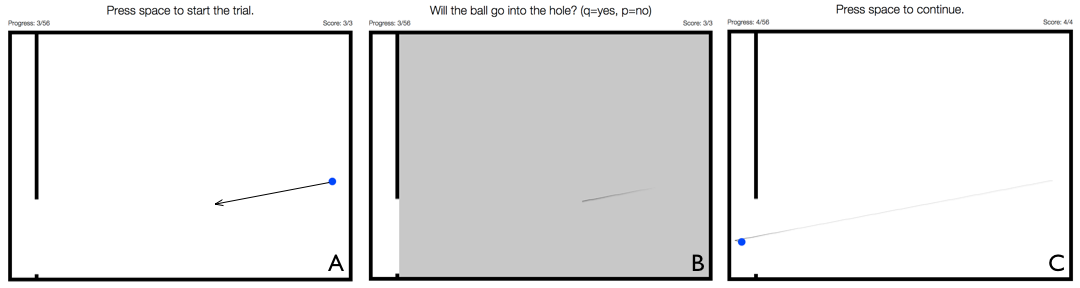
\includegraphics[width=\textwidth]{figures/experiment.png}
        \caption{\textbf{Example experimental trial.} 
        Each panel shows a different part of the trial. 
        \emph{A:} the initial screen presented to the participant.
        The arrow was not part of the actual stimuli; it has been added to reflect the animation that participants observed after pressing ``space''. 
        \emph{B:}  the screen is occluded after observing the stimulus presentation. 
        The faded gray line shows the path the ball took during the initial presentation. 
        \emph{C:} the final position of the ball, after observing the feedback. 
        As in the middle panel, the faded gray line shows the path of the ball.}
        \label{fig:experiment}
    \end{center}
\end{figure*}

%% Plan of the paper
Drawing on the results from both physical simulation and decision-making, we hypothesize that people make predictions by running mental simulations, and that they vary the number of simulations based on their uncertainty.
In this paper, we first formalize our model, combining the simulation model from \citeA{Smith:2013fc} with the \textsc{sprt} decision strategy. 
Next, we describe an experiment in which we asked participants to respond to the question of, ``will the ball go through the hole?'', and analyze peoples' judgments and response times. 
We then demonstrate that our model can explain the empirical pattern of responses and response times we observed. 
Finally, we discuss the implications of our results on the broader, underlying question: how should people make use of mental simulations?

\section{Making decisions from mental simulations}

Consider the task in Figure \ref{fig:experiment}, in which people observe a ball moving inside a box, and must predict whether it will go through the hole.
How do people solve this problem?
Here, we formalize a model that answers this question by combining noisy physical simulations with a decision-making strategy known as the \emph{sequential probability ratio test}, or \textsc{sprt}.

\subsection{Modeling physical simulation}

There is a growing body of evidence that people reason about physical scenes like the one in Figure \ref{fig:experiment} by running noisy simulations.
This hypothesis, referred to as the ``noisy Newton'' hypothesis \cite{Sanborn2013}, states that people have approximate knowledge of physical laws instantiated in a runnable model of intuitive physics.
Using this model, they can extrapolate the future by running a series of noisy simulations \cite{Smith:2013fc,Battaglia2013,Smith:2013ug,Smith:2013th,Smith:2014tx,Ullman:2014ut,Hamrick:2015}.

\citeA{Smith:2013fc} investigated the various sources of uncertainty in these simulations, finding that people's judgments were best captured by a model that took into account both perceptual uncertainty (noise in object locations and their trajectories) and dynamic uncertainty (noise in the object's motion---e.g., a textured floor would cause a ball to deviate from a straight line).
Using this model, we hypothesize that people reason about the task in Figure \ref{fig:experiment} by running noisy physical simulations to estimate where the ball will go.

\subsection{The \textsc{sprt} strategy}

If people are running simulations to reason about physical scenes, then how many simulations do they run?
Because the simulations are noisy, it might be beneficial to run multiple simulations in order to get a better estimate of the outcome.
However, each simulation comes with a time cost.
To optimize this speed-accuracy tradeoff, we apply the \emph{sequential probability ratio test}, or \textsc{sprt} \cite{wald1947sequential} to the samples drawn from the physical simulation.
By combining these two models, we can make predictions both for people's judgments, and how long they take to make those judgments.

We consider binary (or two-alternative forced choice) decisions, where an agent must choose one of two hypotheses, $H_0$ or $H_1$.
In the case of the task in Figure \ref{fig:experiment}, $H_1$ is the hypothesis that the ball goes in, and $H_0$ is the hypothesis that it does not. 
The agent may take samples $X_i$ from a Bernoulli distribution with an unknown parameter $p$ (the probability of sampling evidence for $H_1$), and from these samples estimate the probability that $H_1$ is correct: $\hat{p}=\frac{1}{N}\sum_{i=1}^N X_i$, where $N$ is the total number of samples. 
Then, the decision rule which minimizes the probability of error is $\hat{H}(X_1,\ldots{},X_N)=H_0$ when $\hat{p}<0.5$ and $\hat{H}(X_1,\ldots{},X_N)=H_1$ when $\hat{p}>0.5$.

\begin{figure*}[t]
    \begin{center}
        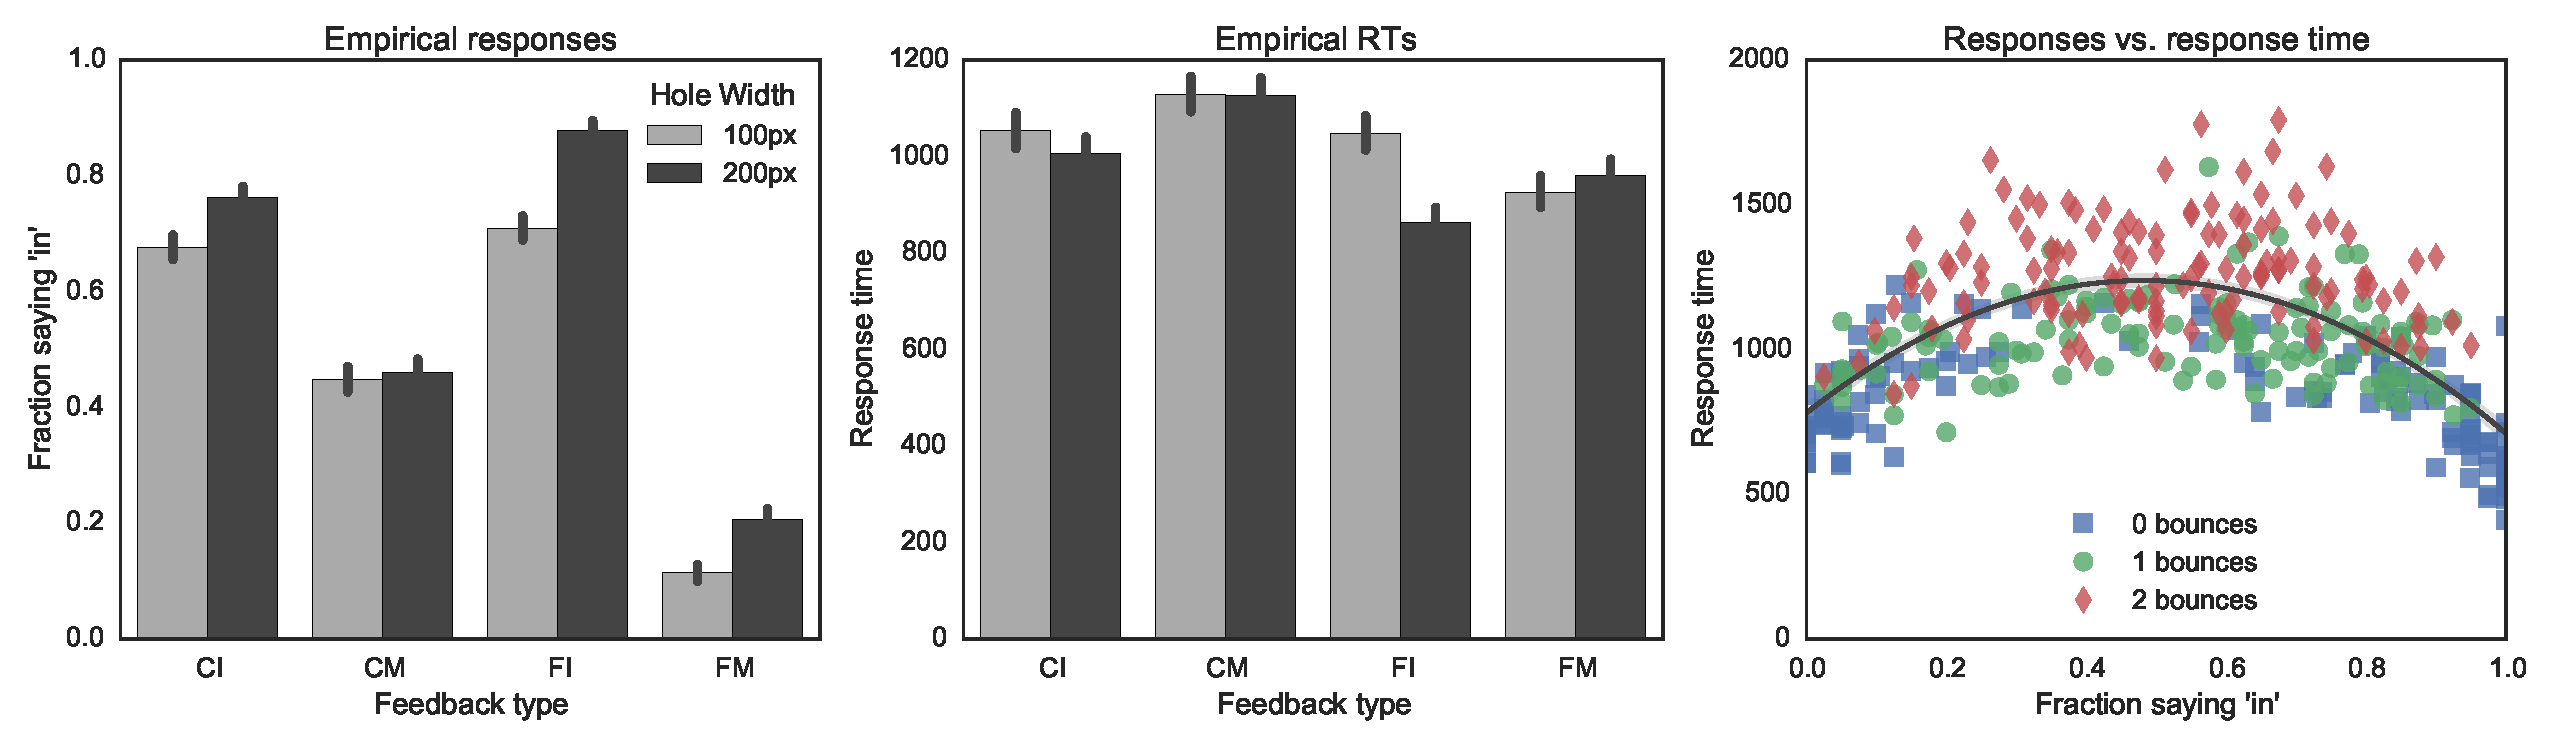
\includegraphics[width=\textwidth]{figures/hole_empirical_results.pdf}
        \caption{\textbf{Response characteristics as a function of trial type.}
        \emph{A:} each bar shows the proportion of participants saying that the ball will go in the hole for a particular trial type ($x$-axis) and hole size (color).
        \emph{B:} like the left subplot, but the $y$-axis shows bootstrapped logarithmic means of RTs. 
        \emph{C:} each point corresponds to a different stimulus, trial type, and hole size.  
        The $x$-axis is the proportion of participants saying the ball will go in the hole, and the $y$-axis is the logarithmic mean RT. 
        The black line indicates a 2nd-order polynomial fit between responses and RTs and the shaded gray region indicates the 95\% confidence interval around the fit.}
        \label{fig:pct-vs-rt}
    \end{center}
\end{figure*}

In the best possible case, the agent takes infinitely many samples and chooses the \emph{maximum a posteriori} (MAP) hypothesis with probability $p$. 
In practice, the agent cannot take infinitely many samples. 
Thus, to determine when to stop sampling (i.e., what the value of $N$ is), the agent continues to sample until the net evidence $Y_N$ reaches some threshold, either $Y_N=T$ to select in favor of $H_1$ or $Y_N=-T$ to select in favor of $H_0$. 
The net evidence is the sum of samples in favor of $H_1$ minus those in favor of $H_0$, or $Y_N=\sum_{i=1}^N 2X_i-1$.

Independent of the actual number of samples taken, the probability of choosing the MAP hypothesis ($H_1$) is:
\begin{equation}
\Pr[\hat{H}(Y_N)=H_1\,|\,H_1,T,p]=\frac{p^T}{p^T+(1-p)^T},
\label{eq:pr-choose-h1}
\end{equation}
and the expected number of samples taken before reaching either $Y_N=T$ or $Y_N=-T$ is given by:
\begin{equation}
\mathbb{E}[N\,|\,T,p]=\frac{T}{1-2p}-\frac{2T}{1-2p}\cdot{}\frac{1-((1-p)/p)^T}{1-((1-p)/p)^{2T}},
\label{eq:expsamp}
\end{equation}
which is derived by \citeA[ch.~XIV, eq. 3.4]{Feller:1968ut}.

\subsection{Combining simulation and \textsc{sprt}}

In order to combine simulation and \textsc{sprt}, we used the model from \citeA{Smith:2013fc} to sample possible trajectories of the ball, from which we estimated a truncated normal posterior predictive distribution of where the ball will go.
From this distribution, we compute the probability $p$ that the ball goes in the hole as the probability mass overlapping the hole.
This probability can then be used to compute Equations \ref{eq:pr-choose-h1} and \ref{eq:expsamp}, which give a formal hypothesis for what decisions people make, and how long it takes them.

Because our experiment (described in the next section) was performed online, we needed to fit the parameters of the model from \citeA{Smith:2013fc} to reflect these different viewing conditions.
To do this, we performed an online replication of the experiment from \citeA{Smith:2013fc} in which we asked people to catch a ball like the one in Figure \ref{fig:experiment} using a paddle that could move up and down along the $y$-axis (see Appendix).
If we assume participants in this auxiliary experiment took on average $M$ samples, then the standard deviation of their judgments ($\sigma_{judgments}$) is not equal to the standard deviation of their simulations ($\sigma_{sims}$), but is instead related by the equation: $\sigma_{judgments} = \sigma_{sims} / \sqrt{M}$.
Therefore, to estimate $\sigma_{sims}$, we allowed for a free parameter, $\sigma_{adj}=\sqrt{M}$, which multiplied our original estimate of the standard deviation.

\section{Testing the \textsc{sprt} model of mental simulation}

To determine whether people choose simulations in a way consistent with \textsc{sprt}, we ran an experiment in which people made a binary judgment about whether a ball traveling across a computer screen would go through a hole (see Figure \ref{fig:experiment}).
We designed the trials to elicit a range of responses by varying the margin by which the ball either missed or went through the hole.
According to \textsc{sprt}, when people's simulations are uncertain---i.e., when the probability that the ball goes in the hole is close to $p=0.5$, such as when the ball just barely goes through the hole---they should be slower to respond.
People should be faster to respond when their simulations are more certain, such as when the ball misses the hole by a wide margin.

\subsection{Participants}

We recruited \HoleNumComplete{} participants on Amazon's Mechanical Turk using the psiTurk \cite{McDonnell12} experimental framework.
Participants were treated in accordance with UC Berkeley IRB standards and were paid \$0.60 for 6.5 minutes of work.
Participants were randomly assigned to one of eight conditions, which determined which stimuli they judged (see Stimuli). 
We excluded \HoleNumFailed{} participants for answering incorrectly on more than one control trial (see Stimuli), leaving a total of \HoleNumOk{} participants.

\subsection{Procedure}

On each trial, participants were shown the scene, including the initial position of the ball and the location of the hole. 
Participants were instructed to press ``space'' to begin the trial, after which an animation of the initial stimulus began (see Stimuli). 
As soon as this animation concluded, a gray box was drawn over the screen, occluding the ball (but not the line depicting the path it had traveled so far; this was left in as a reminder of where the ball had come from). 
Participants were asked, ``will the ball go in the hole?'', and were instructed to press `q' if they thought it would, and `p' otherwise. 
After responding, text appeared saying ``Correct!'' or ``Incorrect.''
The gray occluder was removed, and participants were shown a feedback animation of the path of the ball (see Stimuli).
The final frame of this animation remained on the screen until participants pressed ``space'' to advance to the next trial.

Participants were given seven instruction trials prior to the experiment to familiarize them with the procedure.
Then, participants made judgments on 48 experimental trials in a random order.
There were also eight control trials, which were shown in a random order after every seven experiment trials.

\begin{figure*}[t]
    \begin{center}
        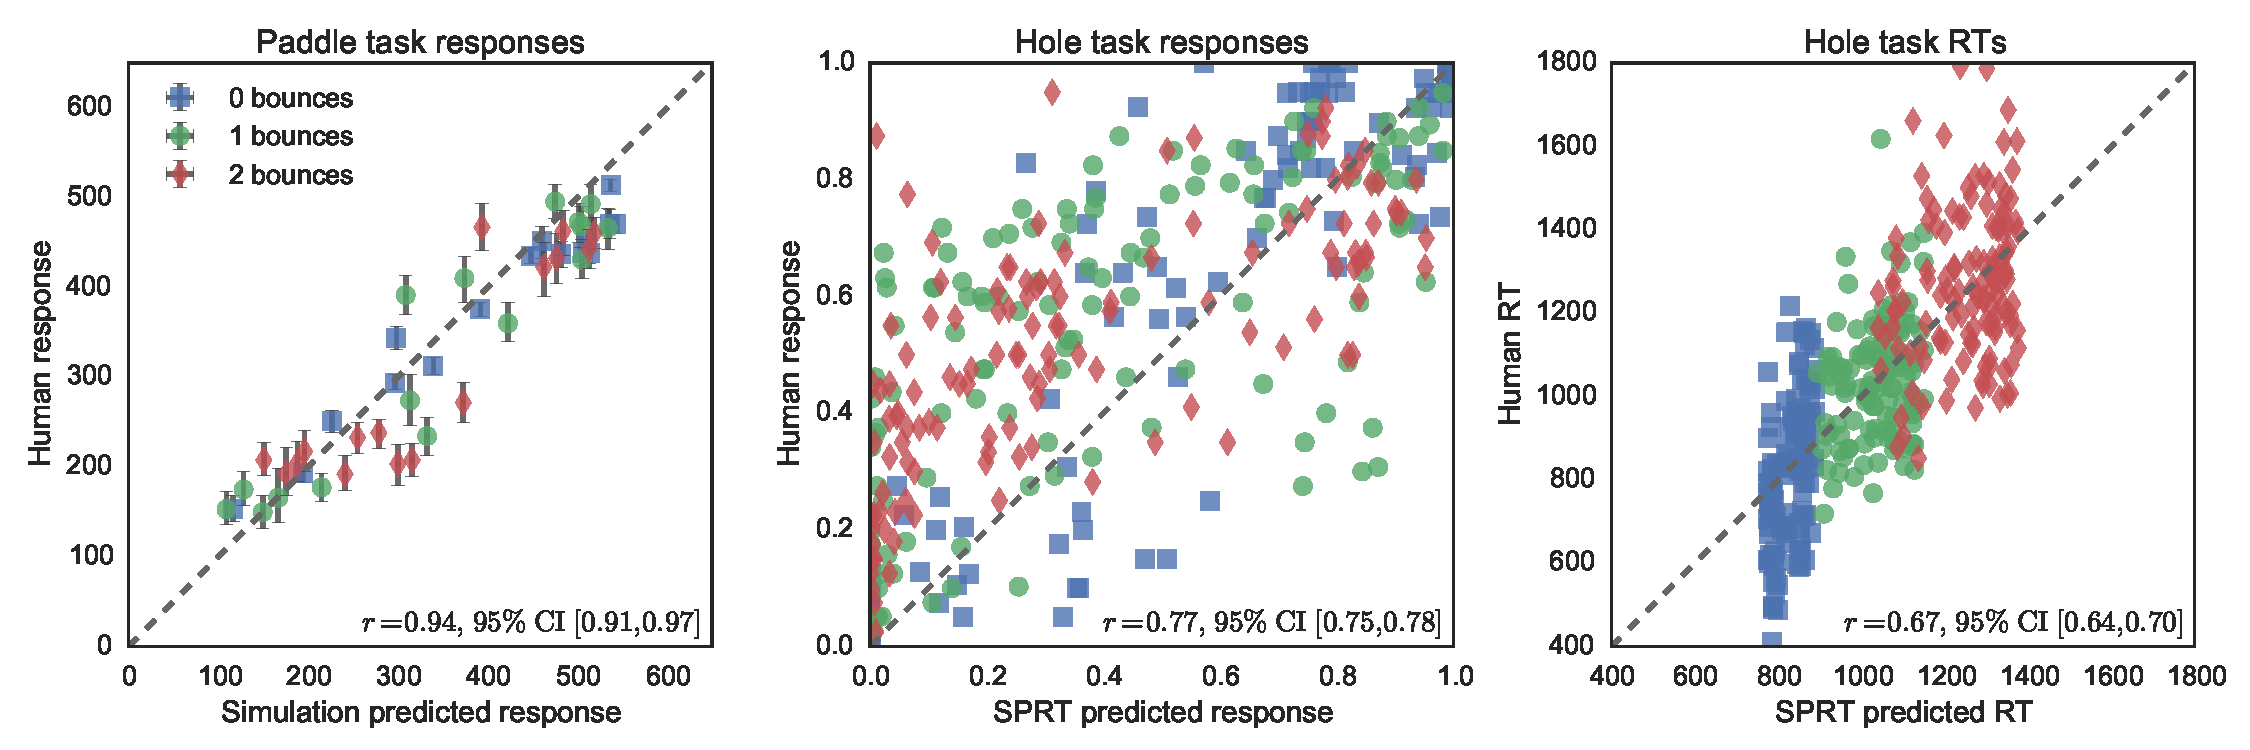
\includegraphics[width=\textwidth]{figures/model_results.pdf}
        \caption{\textbf{Model vs. human comparison.} 
        In both plots, each point corresponds to a different stimulus, trial type, and hole size. 
        Dashed lines indicate perfect correspondence between model and people. 
        \emph{A:} The $x$-axis is the probability the model says the ball will go in the hole, and the $y$-axis is the proportion of participants saying the ball will go in the hole. 
        \emph{B:} Color and shape indicate the number of times the ball bounced during feedback. 
        The $x$-axis is the model RTs, and the $y$-axis is the logarithmic mean RTs of participants.}
        \label{fig:model-results}
    \end{center}
\end{figure*}

\subsection{Stimuli}

The stimuli consisted of two animations---the \emph{stimulus presentation} and the \emph{feedback} animations---depicting a blue ball with a radius of 10px moving in a box with dimensions 900px $\times$ 650px.
In both animations, the ball had a velocity of 400px/s, and as it moved, it traced a gray line (see Figure \ref{fig:experiment}).
The stimulus presentation had a duration of 0.775s and depicted the ball moving in a particular direction.
The feedback had a duration of 1.5s and picked up where the stimulus presentation left off; it showed the ball either going into the hole or bouncing off the wall that contained the hole for.
Across all stimuli, the ball traveled the same distance during both animations, and could bounce on the other walls 0, 1, or 2 times before going into the hole or hitting the wall with the hole.

There were 48 different initial animations, equally balanced by number of bounces during feedback (16 each for 0, 1, and 2 bounces). 
For each of these initial animations, there were four trial types and two hole sizes, for a total of eight versions of each stimulus. 
The four trial types were: ``far in'' (FI), where the ball went through the center of the hole; ``far miss'' (FM), where the ball missed the hole by a wide margin; ``close in'' (CI), where the ball just barely went through the hole; and `` close miss'' (CM), where the ball just barely missed the hole. 
The two hole sizes were 100px and 200px.

In order to ensure that participants never saw the same initial animation twice, we used a latin-square design of Initial Animation $\times$ Trial Type $\times$ Hole Size.
Thus, each participant saw each initial animation once, each trial type 12 times, and each hole size 24 times.
This also ensured that the ball would go through the hole half the time, so that participants would not be biased to respond either way.
Additionally, there were seven instruction trials and eight control trials, which were the same for all participants.
The control trials were designed to be easy and were either of type ``straight hit'' (with a hole size of either 300px or 350px) or ``far miss'' (with a hole size of 100px).
Thus, participants saw a total of 63 trials.

\subsection{Results}

\subsubsection{Responses}

On average, participants were correct \AvgCorrect{} of the time and responded that the ball would go in the hole \AvgResponse{} of the time (\ResponseN{}), excluding catch trials.
There was a significant effect of trial type on participants' responses (\ResponseHoleClass{}) as well as a significant effect of hole size (\ResponseHoleSize{}).
There was also an interaction between trial type and hole size (\ResponseFull{}).
There was a significant difference between responses for the two hole sizes (for CI, \ResponseCIttest{}; for FI, \ResponseCIttest{}; and for FM, \ResponseFMttest{}) except on the CM trials (\ResponseCMttest{}).
Figure \ref{fig:pct-vs-rt}A shows responses as a function of trial type and hole size.

\subsubsection{Response times}

For all analyses of response time (RT), we computed averages using bootstrapped logarithmic means (exponential of the mean of the log RTs), using 10000 bootstrap samples.
On average, participants responded in \AvgRT{}, excluding catch trials.
There were effects of both trial type (\RTHoleClass{}) and hole size (\RTHoleSize{}), as well as an interaction between trial type and hole size (\RTFull{}).
As in Figure \ref{fig:pct-vs-rt}B, hole size only had an effect in the case of the FI trials (\ResponsetimeFIttest{}; for CI, \ResponsetimeCIttest{}; for CM, \ResponsetimeCMttest{}; and for FM, \ResponsetimeFMttest{}).

Participants were fastest to respond on trials with zero bounces (\RTZeroBounces{}), slower to respond on trials with one bounce (\RTOneBounces{}), and slowest to respond on trials with two bounces (\RTTwoBounces{}).

\subsubsection{Relationship of responses and RTs}

According to \textsc{sprt}, participants should be slower on trials for which they are less certain (i.e., when their average response is closer to 0.5), and faster when they are more certain (i.e., when their average response is closer to 0 or 1).
Figure \ref{fig:pct-vs-rt}C illustrates that this trend does indeed appear.
To demonstrate this more quantitatively, we fit both 1st- and 2nd- order polynomial functions to the relationship between responses and RTs.
The 1st-order function had \AicFirstOrder{} and \BicFirstOrder{}, while the 2nd-order function had \AicSecondOrder{} and \BicSecondOrder{}.

Participants' responses do not fully account for their RTs, however: the number of bounces is also a strong predictor of RT.
Although people do make more variable predictions as bounces are added \cite{Smith:2013fc}, and more variable trials have longer RTs, there appears to be an additional time cost.
We modified the 2nd-order polynomial to include the number of bounces as an regressor, and found that the number of bounces is a strong predictor of RT above and beyond the responses (with bounces, \AicSecondOrderWithBounces{} and \BicSecondOrderWithBounces{}; without bounces, \AicSecondOrder{} and \BicSecondOrder{}).
From the coefficient, we find that the each bounce adds \RTBounceCoef{}.
Thus, even if people are using a \textsc{sprt}-like strategy, there is a time cost per bounce that cannot be explained by simulation variance alone.
This suggests that there is a discrepancy between our simulation model and the manner in which people are \emph{actually} running simulations; investigating the details of this discrepancy is an area for future work.

\subsubsection{Learning}

To check for practice effects, we computed Spearman rank correlations (with 95\% confidence intervals computed from 10000 bootstrap samples) between trial number and accuracy, as well as between trial number and RT.
We found an overall effect of practice on accuracy (\ResponseTrialCorr{}), though in the second half of the experiment, this effect disappeared (\ResponseTrialCorrLate{}).
There was also an overall effect of practice on RT (\RTTrialCorr{}), which was strong both in the first (\RTTrialCorrEarly{}) and second (\RTTrialCorrLate{}) halves of the experiment.
Future work will need to include a longer training period to alleviate these practice effects.

\subsubsection{Model comparison}

\begin{table}
    \centering
    \begin{tabular}{ccl}
    \toprule
    \textbf{Model} & \textbf{Bounces} & \textbf{Correlation} \\
    \midrule
    $T=1$ & 0   & \NoSamplesHoleRTCorrZeroBounces{} \\
          & 1   & \NoSamplesHoleRTCorrOneBounce{} \\
          & 2   & \NoSamplesHoleRTCorrTwoBounces{} \\
          & all & \NoSamplesHoleRTCorr{} \\
    \midrule
    $T=2$ & 0   & \HoleRTCorrZeroBounces{} \\
          & 1   & \HoleRTCorrOneBounce{} \\
          & 2   & \HoleRTCorrTwoBounces{} \\
          & all & \HoleRTCorr{} \\
    \bottomrule
    \end{tabular}
    \vspace{.25cm}
    \caption{\textbf{Correlations between human and model RTs.} The SPRT model ($T=2$) can capture variations in RTs within bounce conditions, while the single sample model ($T=1$) cannot. Note that the correlations for the $T=1$ model are non-zero because we estimate $\mathbb{E}[B]$ from the simulation model, so there is some variation in the expected number of bounces across stimuli.}
    \label{tbl:rt}
\end{table}

If we assume that every sample takes the same amount of time, RTs as predicted by the model should be directly proportional to $\mathbb{E}[N\,|\,T,p]$.
However, because bounces were a strong predictor of RT, we also incorporated the number of bounces, $B$, according to $RT = \beta_0 + (\beta_1 + \beta_2\cdot{}\mathbb{E}[B]) \cdot{}\mathbb{E}[N\,|\,T,p]$.
Briefly, $\beta_0$ is the time to set up the simulation(s) and to respond, $\beta_1$ is the time to simulate with no bounces, and $\beta_2$ is the time needed to simulate each bounce.
We used the physical simulation model to determine $\mathbb{E}[B]$ as the average number of times the ball bounced across all model simulations.
We then fit all parameters ($T$, $\sigma_{adj}$, $\beta_0$, $\beta_1$, and $\beta_2$) to minimize sum squared error between modeled and observed RTs, using 10000 samples from the physical simulation model.
The best fitting values were: \threshold{}, \sdadj{},\footnote{If \sdadj{}, then $M<1$. How could people be taking less than one sample?
We suspect that $\sigma_{adj}<1$ because the model overestimates the standard deviation of the ball's trajectory; thus, it is likely that people are taking one sample, and $\sigma_{adj}$ is adjusting for inflated uncertainty in the model.} \betazero{}, \betaone{}, and \betatwo{}.

We computed Pearson correlations between the model and people with 95\% confidence intervals computed from 10000 bootstrap samples.
The fitted model explains participants' judgments of whether the ball would go in the hole very well (\HoleResponseCorr{}, see Figure \ref{fig:model-results}A), and is also a good predictor of RT (\HoleRTCorr{}).
A model that takes one sample each time (equivalent to \textsc{sprt} with $T=1$) is slightly better at explaining people's responses (\RawHoleResponseCorr{}), and is equally good at explaining overall RT in terms of correlation (\NoSamplesHoleRTCorr{}).
However, according to both BIC and AIC, the $T=1$ model is slightly worse (\BicNoSamples{} and \AicNoSamples{}) than the full model (\BicFull{} and \AicFull{}) at explaining RTs.
Moreover, the $T=1$ model cannot explain variance in RTs within bounces, whereas the full model with $T=2$ can (see Table \ref{tbl:rt}).
If the number of bounces is excluded, the model with $T=2$ can predict human RTs to a moderate degree (\NoBouncesHoleRTCorr{}), while the model with $T=1$ cannot predict RTs at all.

\section{Discussion}

In this paper, we asked the question: do people optimally use mental simulations?
We hypothesized that people use noisy physical simulations to predict whether a ball would go in a hole, and that they vary the number of simulations in order to exploit the fact that some judgments are easier to make than others.
The results of our experiment paint a clear picture that people \emph{do} vary the number of samples they take, as evidenced by the increase in response time on the trials they were most uncertain about.
Comparing people's responses and response times to those of the model, we found a strong fit.
This provides evidence that people not only rely on approximate physical simulations, but that they vary the number of simulations that they run according to \textsc{sprt}.

If \textsc{sprt} is the optimal strategy, then what is the optimal threshold?
We found the best fitting \textsc{sprt} threshold to be \threshold{}, which is consistent with previous research.
According to \citeA{Vul:2014ba}, a sample-based agent should only take a small number of samples before making a judgment so long as there is any cost to taking samples.
While taking a small number of samples provides a worse chance of making a good decision than taking multiple samples, over the long run, this strategy maximizes expected utility across a large number of judgments.
There has been some evidence that this story also holds true for mental simulations.
For example, \citeA{Battaglia2013} analyzed the variability of people's responses in tasks concerning towers of building blocks, and found that participants seemed to use between three and seven samples per judgment.
However, this paper is the first to provide evidence not only that people use a small number of simulations, but that they vary the number of simulations in response to task demands.

Mental simulation is a powerful and flexible tool, as it offers a way to make predictions about scenarios that have not yet (or may never) come to pass.
In this work, we demonstrated that when people use mental simulation, they are sensitive to their own uncertainty in reasoning about the task and accordingly adjust how many simulations they run.
This results joins others \cite<e.g.>{Hamrick:2014wq} in explaining not just \emph{that} people use simulation to reason about the world, but \emph{how} they use it.
While there are still many questions left unanswered---e.g., how do people use simulations in non-binary tasks?---this work brings us one step closer to understanding of how mental simulation is used.

\subsection{Acknowledgments}

This work was supported by a NSF GRF awarded to JBH, a UCSD Chancellor’s Interdisciplinary Collaboratories grant awarded to KAS, NSF CPS grant 1239323, and \TODO{}.

\section{Appendix: Replication of \citeA{Smith:2013fc}}

\subsubsection{Participants}

We recruited \PaddleNumComplete{} participants using psiTurk \cite{McDonnell12}.
Participants were treated in accordance with UC Berkeley IRB standards and were paid \$0.60 for 5 minutes of work.
We excluded \PaddleNumFailed{} people for failing to catch the ball on more than one control trial.

\subsubsection{Stimuli}

The stimuli were modified versions of those used in the main experiment, with two differences.
First, instead of a wall with a hole in it, there was a paddle of length 100px that could move up and down the $y$-axis.
Second, instead of a full feedback animation, we just displayed the last frame.
Because there was no hole that could vary by trial, there were only 48 stimuli, plus seven instruction and eight catch trials.

\subsubsection{Procedure}

Like the main experiment, there were two phases: the training phase and the experimental phase.
On each trial, participants were shown the scene, including the initial position of the ball.
The paddle begin at the center of the $y$-axis, and was freely movable at the start of the trial.
Participants were instructed to press ``space'' to begin the trial and display the stimulus animation.
After the stimulus presentation, a gray occluder appeared, as well as a timer that began counting down for 2 seconds.
During this time, participants had to move the paddle to catch the ball in the position it would be when the timer was up.
When the timer finished, the paddle froze, the occluder was removed, and the full path of the ball was revealed.
Participants were told whether they caught the ball or not, and then instructed to press ``space'' to begin the next trial.

\subsubsection{Results}

We fit the model parameters of $\sigma_p$, $\kappa_v$, $\kappa_m$, $\kappa_b$, and $\sigma_0$ to participant's responses \cite<for details, see>{Smith:2013fc}, finding the best fitting parameters to be \perr{}, \kapv{}, \kapm{}, \kapb{}, and \sdzero{}.
With these parameters, we found very similar results to those from \citeA{Smith:2013fc}.
In particular, we found a correlation of \PaddleCorr{} between the model's predicted means of where the ball would end up and people's average location of the paddle.

\bibliographystyle{apacite}
\renewcommand{\bibliographytypesize}{\small}
\setlength{\bibleftmargin}{.125in}
\setlength{\bibindent}{-\bibleftmargin}
\bibliography{references}

\end{document}
